%!TEX root = practicum4.tex
Since the Voronoi diagram is the dual of the Delaunay Triangulation, taking the dual of the second gives the first. The duals of the different parts that make up a doubly connected edge list are given in \autoref{tab:c:duals}.

\begin{table}
	\centering
	\begin{tabular}{ll}
		Voronoi diagram 	& Delaunay Triangulation\\
		\hline
		\hline
		Face 				& Vertex\\
		\hline
		circumcentre 		& origin\\
		outer component 	& incident edge\\
		\hline
		Vertex 				& Face\\
		\hline
		origin 				& circumcentre\\
		incident edge 		& outer component\\
		\hline
		Edge 				& Edge\\
		\hline
		origin 				& incident face\\
		incident face 		& destination\\
		twin 				& twin\\
	\end{tabular}
	\caption{The dual of the elements of the DCEL.}
	\label{tab:c:duals}
\end{table}

The code used to determine the duals of the elements of a DCEL is presented in \autoref{lst:c:dual}. To set the twins I have used the local method \t{set_twins()} which uses the fact that edges $e$ and their twins $e'$ are placed in the list in the following order: $e_1$, $e_1'$, $e_2$, $e_2'$, $\ldots$.

\lstinputlisting[firstline=138, lastline=168, label={lst:c:dual}, caption={The method \t{dual} in the class \t{DCEL}.}]{../dcel.py}

Since I could not figure out what the dual of the next and previous edges where I have used written the method \t{set_next_and_previous()}. For each \t{Face} in the \t{DCEl} this method find the edges adjoining that face and sorts out the next and previous using the coordinates of their vertices. \t{Face}s are joined to the \t{DCEL} using the method \t{add_face()} which checks for duplicates before adding the \t{Face}, see \autoref{lst:c:add_face}.

\lstinputlisting[firstline=114, lastline=121, label={lst:c:add_face}, caption={The method \t{add_face} in the class \t{DCEL}.}]{../dcel.py}

Thus by taking the dual, and some searching in lists in this case, on can generate a Voronoi diagram based on a Delaunay triangulation without geometric operations.\\

A Voronoi diagram created by taking the dual of the Delaunay Triangulation is presented in \autoref{fig:c:voronoi}. The Boundaries of a simpler Voronoi diagram are highlighted in \autoref{fig:c:voronoi_small} to show that every half-edge of an outer non-finite face is shown. 

\begin{figure}
	\begin{minipage}[t]{0.45\textwidth}
		\centering
		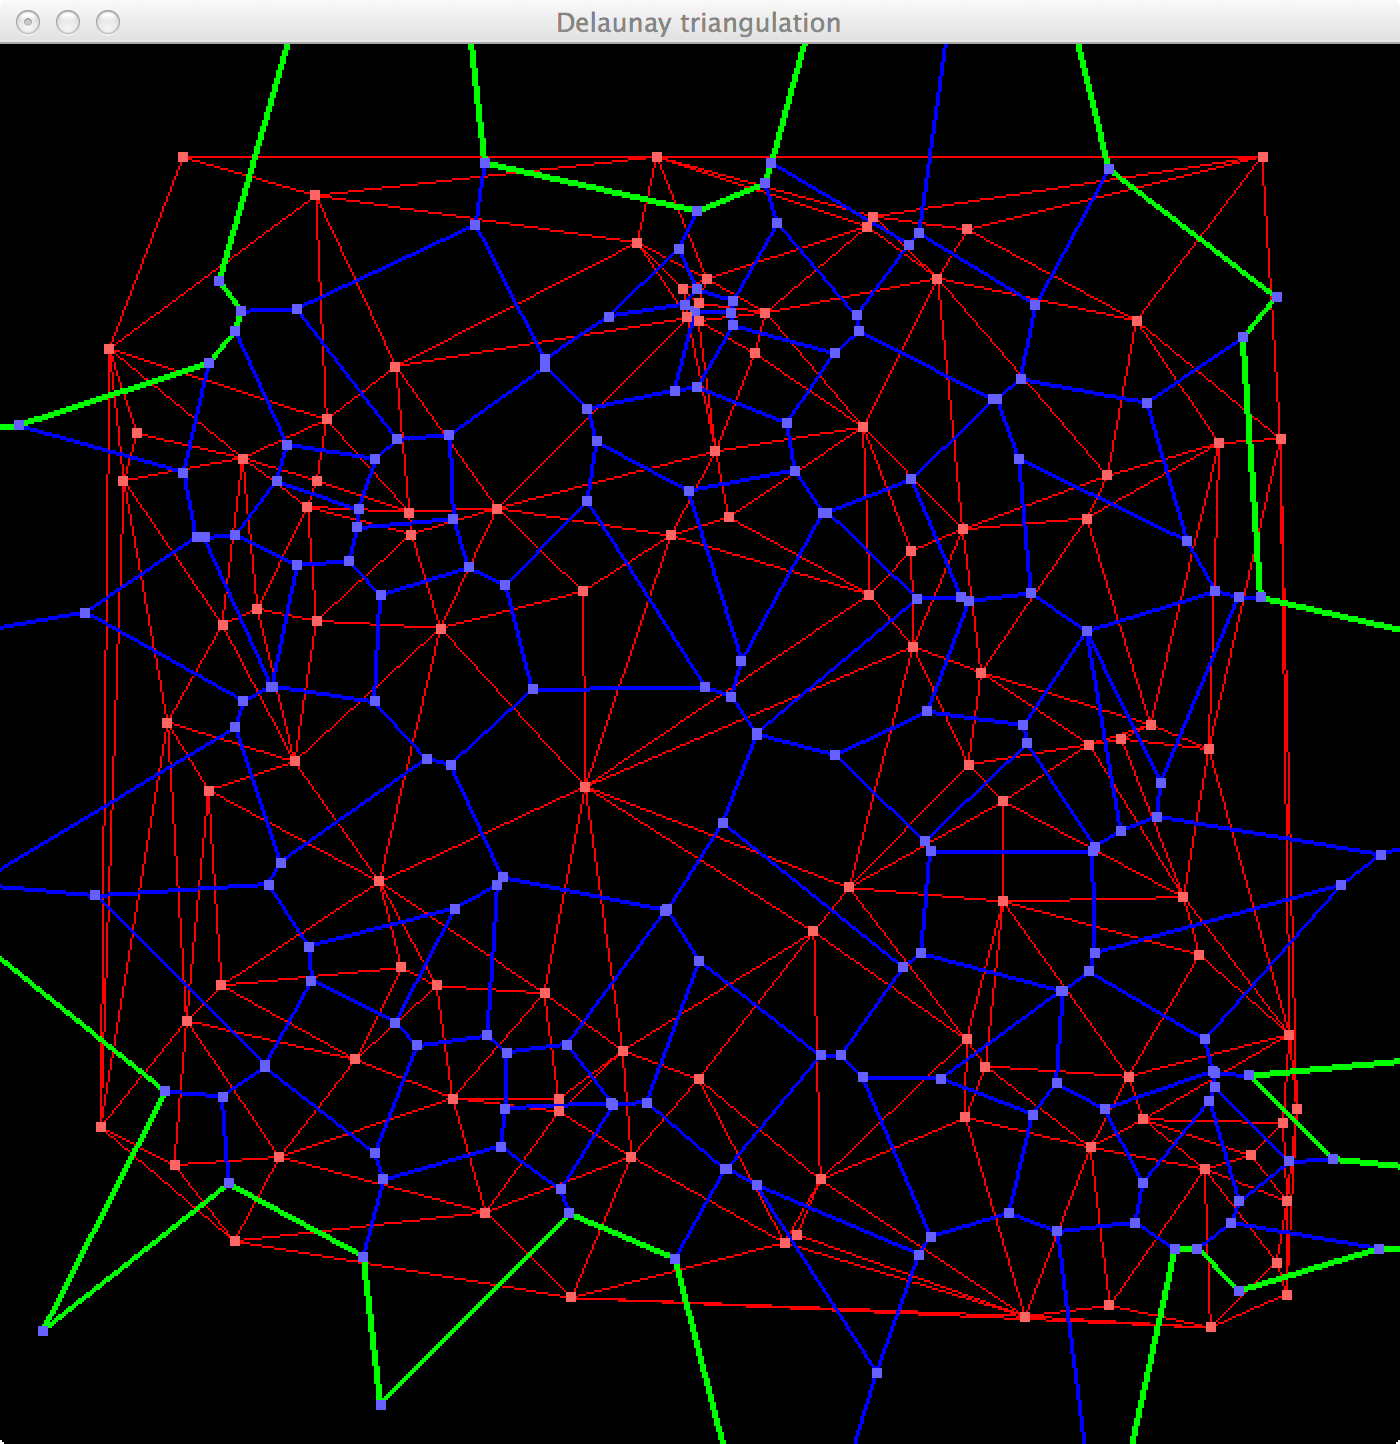
\includegraphics[width=0.9\textwidth]{./img/c_voronoi}
		\caption{A Voronoi diagram, shown in blue and green, based on the Delaunay triangulation shown in red.}
		\label{fig:c:voronoi}		
	\end{minipage}
	\hspace{0.1\textwidth}
	\begin{minipage}[t]{0.45\textwidth}
		\centering
		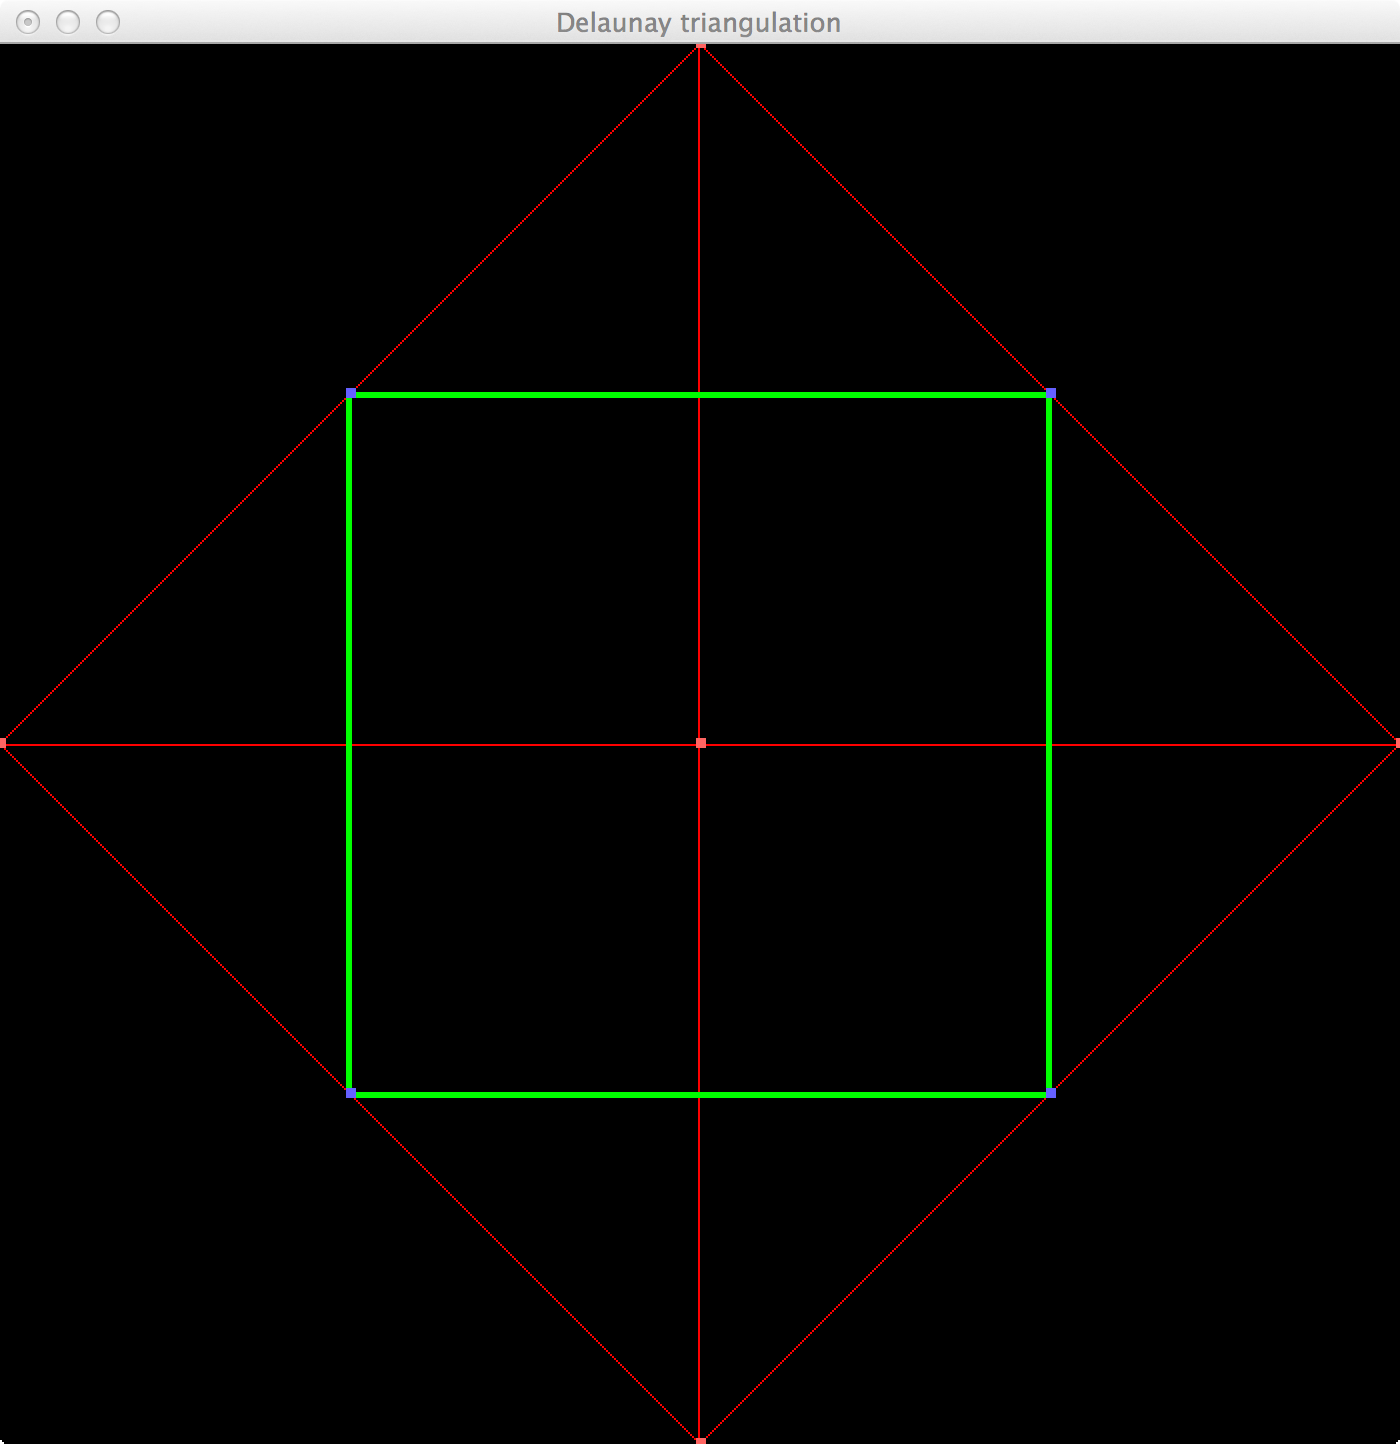
\includegraphics[width=0.9\textwidth]{./img/c_small_triangulation}
		\caption{A Voronoi diagram, shown in blue, with edges highlighted in green, based on the Delaunay triangulation shown in red.}
		\label{fig:c:voronoi_small}		
	\end{minipage}
\end{figure}

The outer boundaries are found with the following algorithm:
	\begin{enumerate}
		\item Find a infinite \t{HalfEdge} \t{edge} with its \t{origin} on the outer edge of the diagram.
		\item Store the origin of this \t{HalfEdge} as \t{first_vertex}.
		\item \t{while} the destination of \t{edge} is not the \t{first_vertex}:
			\begin{enumerate}
				\item If \t{edge} is infinite get the next of its twin.
				\item Else store edge \t{edge} as part of the outer boundary and continue with the next of \t{edge}.
			\end{enumerate}
		\item Store \t{edge} as part of the outer boundary.
	\end{enumerate}

Which is implemented in \autoref{lst:c:get_outer_boundary_of_voronoi}. The code used to present the results is shown in \autoref{lst:c:display_delaunay_and_voronoi}. To run the script with this display code use the option \t{-voronoi}.

\lstinputlisting[firstline=123, lastline=136, label={lst:c:get_outer_boundary_of_voronoi}, caption={The method \t{get_outer_boundary_of_voronoi} in the class \t{DCEL}.}]{../dcel.py}

\lstinputlisting[firstline=194, lastline=239, label={lst:c:display_delaunay_and_voronoi}, caption={The method \t{display_delaunay_and_voronoi} in the script \t{assignmetn4A}.}]{../assignment4A.py}

